\documentclass[11pt,oneside]{book}

\usepackage[margin=1in]{geometry}
\usepackage[T1]{fontenc}
\usepackage[utf8]{inputenc}
\usepackage{lmodern}
\usepackage{microtype}
\usepackage{amsmath,amssymb,mathtools,bm}
\usepackage{booktabs,tabularx,array,longtable}
\usepackage{enumitem}
\usepackage{xcolor}
\usepackage{hyperref}
\usepackage[most]{tcolorbox}
\usepackage{tikz}
\usepackage{pgfplots}
\usepackage{tikz-3dplot}
\usepackage{float}
\usepackage{caption}
\usepackage{fancyhdr}
\usepackage{listings}

\pgfplotsset{compat=1.18}
\usetikzlibrary{arrows.meta,calc,positioning,patterns,decorations.pathreplacing,fit,backgrounds,shadows.blur,matrix}
\usepgfplotslibrary{fillbetween}

\definecolor{chapterblue}{HTML}{1F5AA6}
\definecolor{chapterteal}{HTML}{168A8F}
\definecolor{chapterorange}{HTML}{D9822B}
\definecolor{chaptergreen}{HTML}{2D8A4E}
\definecolor{chapterpurple}{HTML}{6B4EAA}
\definecolor{chapterred}{HTML}{B23B3B}
\definecolor{softblue}{HTML}{EAF3FF}
\definecolor{softgreen}{HTML}{EAF8EF}
\definecolor{softorange}{HTML}{FFF4E6}
\definecolor{softpurple}{HTML}{F3EEFF}
\definecolor{softred}{HTML}{FFF0F0}
\definecolor{softgray}{HTML}{F6F7F9}
\definecolor{darkgray}{HTML}{30343B}

\hypersetup{
  colorlinks=true,
  linkcolor=chapterblue,
  urlcolor=chapterblue,
  citecolor=chapterblue,
  pdftitle={Chapter 25: Multivariable Calculus for Data Science and Machine Learning},
  pdfauthor={}
}

\setlength{\parindent}{0pt}
\setlength{\parskip}{0.65em}
\setlength{\headheight}{14pt}
\setlist[itemize]{topsep=2pt,itemsep=2pt}
\setlist[enumerate]{topsep=2pt,itemsep=2pt}

\pagestyle{fancy}
\fancyhf{}
\lhead{\small Chapter 25. Calculus for Data Science and Machine Learning}
\rhead{\small \thepage}
\renewcommand{\headrulewidth}{0.4pt}

\newcommand{\R}{\mathbb R}
\newcommand{\grad}{\nabla}
\newcommand{\norm}[1]{\left\lVert #1\right\rVert}
\newcommand{\abs}[1]{\left\lvert #1\right\rvert}
\newcommand{\dd}{\,d}
\newcommand{\T}{^{\mathsf T}}
\DeclareMathOperator{\col}{Col}
\DeclareMathOperator{\diag}{diag}
\DeclareMathOperator{\sigmoid}{sigmoid}

\tikzset{
  vector/.style={-Latex,very thick,chapterblue},
  descent/.style={-Latex,very thick,chapterred},
  nodebox/.style={draw=chapterblue!60!black,fill=softblue,rounded corners=2mm,align=center,minimum height=9mm,inner sep=3mm},
  greenbox/.style={draw=chaptergreen!60!black,fill=softgreen,rounded corners=2mm,align=center,minimum height=9mm,inner sep=3mm},
  orangebox/.style={draw=chapterorange!70!black,fill=softorange,rounded corners=2mm,align=center,minimum height=9mm,inner sep=3mm},
  purplebox/.style={draw=chapterpurple!70!black,fill=softpurple,rounded corners=2mm,align=center,minimum height=9mm,inner sep=3mm},
  redbox/.style={draw=chapterred!70!black,fill=softred,rounded corners=2mm,align=center,minimum height=9mm,inner sep=3mm}
}

\newtcolorbox{mainideabox}[1][]{
  enhanced,breakable,
  colback=softblue,
  colframe=chapterblue,
  title=#1,
  fonttitle=\bfseries,
  boxrule=0.8pt,
  arc=2mm,
  left=2mm,right=2mm,top=1mm,bottom=1mm
}

\newtcolorbox{definitionbox}[1][]{
  enhanced,breakable,
  colback=softgreen,
  colframe=chaptergreen,
  title=#1,
  fonttitle=\bfseries,
  boxrule=0.8pt,
  arc=2mm,
  left=2mm,right=2mm,top=1mm,bottom=1mm
}

\newtcolorbox{examplebox}[1][]{
  enhanced,breakable,
  colback=white,
  colframe=chapterblue!75!black,
  colbacktitle=chapterblue!75!black,
  title=#1,
  fonttitle=\bfseries,
  boxrule=0.8pt,
  arc=2mm,
  left=2mm,right=2mm,top=1mm,bottom=1mm
}

\newtcolorbox{tipbox}[1][]{
  enhanced,breakable,
  colback=softorange,
  colframe=chapterorange,
  title=#1,
  fonttitle=\bfseries,
  boxrule=0.8pt,
  arc=2mm,
  left=2mm,right=2mm,top=1mm,bottom=1mm
}

\newtcolorbox{warningbox}[1][]{
  enhanced,breakable,
  colback=softred,
  colframe=chapterred,
  title=#1,
  fonttitle=\bfseries,
  boxrule=0.8pt,
  arc=2mm,
  left=2mm,right=2mm,top=1mm,bottom=1mm
}

\newtcolorbox{summarybox}[1][]{
  enhanced,breakable,
  colback=softpurple,
  colframe=chapterpurple,
  title=#1,
  fonttitle=\bfseries,
  boxrule=0.8pt,
  arc=2mm,
  left=2mm,right=2mm,top=1mm,bottom=1mm
}

\lstset{
  basicstyle=\ttfamily\small,
  keywordstyle=\color{chapterblue}\bfseries,
  commentstyle=\color{chaptergreen!70!black},
  stringstyle=\color{chapterorange!80!black},
  frame=single,
  rulecolor=\color{softgray},
  backgroundcolor=\color{softgray},
  columns=fullflexible,
  keepspaces=true,
  showstringspaces=false
}

\begin{document}
\setcounter{chapter}{24}
\chapter{Multivariable Calculus for Data Science and Machine Learning}

\begin{mainideabox}[Chapter overview]
Machine learning training is an optimization problem on a high-dimensional parameter space. A model turns inputs into predictions, a loss function turns prediction errors into a single number, and calculus tells us how that number changes as the parameters move. The main objects are familiar: gradients, Jacobians, Hessians, chain rules, tangent approximations, and level sets. What changes in modern data science is scale: instead of two or three variables, the parameter vector may contain thousands, millions, or billions of components.
\end{mainideabox}

\section*{Learning goals}
By the end of this chapter, you should be able to:
\begin{enumerate}
  \item translate a learning problem into a multivariable function of parameters;
  \item identify loss functions, empirical risk, gradients, Jacobians, and Hessians;
  \item derive gradients for linear regression, logistic regression, and simple neural-network models;
  \item interpret gradient descent as motion on a high-dimensional surface;
  \item explain the role of regularization in optimization and statistical learning;
  \item use computational visualization to study loss landscapes and gradient-based training;
  \item connect calculus ideas to automatic differentiation, backpropagation, and modern AI workflows.
\end{enumerate}

\begin{figure}[H]
\centering
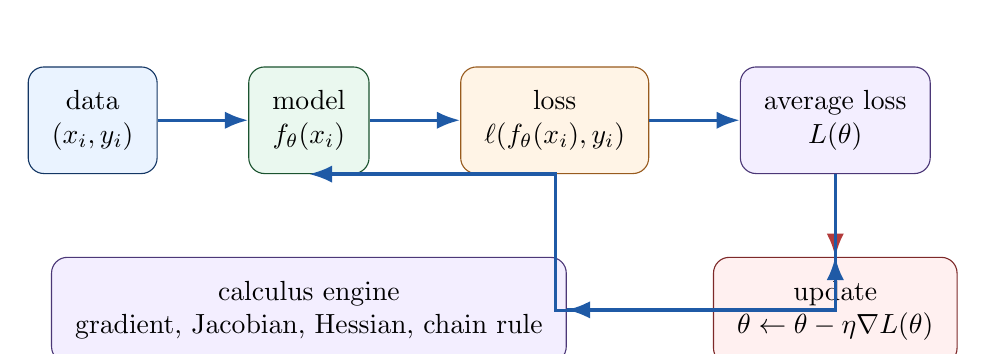
\begin{tikzpicture}[node distance=1.05cm and 1.15cm]
  \node[nodebox] (data) {data\\$(x_i,y_i)$};
  \node[greenbox,right=of data] (model) {model\\$f_\theta(x_i)$};
  \node[orangebox,right=of model] (loss) {loss\\$\ell(f_\theta(x_i),y_i)$};
  \node[purplebox,right=of loss] (risk) {average loss\\$L(\theta)$};
  \node[redbox,below=of risk] (update) {update\\$\theta\leftarrow \theta-\eta\grad L(\theta)$};
  \node[purplebox,below=of model] (calc) {calculus engine\\gradient, Jacobian, Hessian, chain rule};
  \draw[vector] (data) -- (model);
  \draw[vector] (model) -- (loss);
  \draw[vector] (loss) -- (risk);
  \draw[descent] (risk) -- (update);
  \draw[vector] (risk) |- (calc);
  \draw[vector] (calc) -| (update);
  \draw[vector] (update.west) -- ++(-2.0,0) |- (model.south);
\end{tikzpicture}
\caption{A supervised learning workflow viewed as multivariable calculus. The parameter vector $\theta$ is adjusted by information from derivatives of the loss.}
\end{figure}

\section{Why machine learning is multivariable calculus}

A supervised learning problem begins with data
\[
(x_1,y_1),(x_2,y_2),\ldots,(x_n,y_n),
\]
where each input $x_i$ is often a vector in $\R^d$ and each output $y_i$ may be a number, a class label, or another vector. A model is a family of functions
\[
f_\theta:\R^d\to\R^m,
\]
where $\theta\in\R^p$ is a vector of parameters. Training the model means choosing $\theta$ so that $f_\theta(x_i)$ is close to $y_i$ for the observed data and hopefully remains accurate on new data.

The central object is a \emph{loss function}
\[
L(\theta)=\frac1n\sum_{i=1}^n \ell(f_\theta(x_i),y_i),
\]
a function from parameter space to the real line:
\[
L:\R^p\to\R.
\]
So training is not mysterious from the viewpoint of calculus: it is optimization for a function of many variables.

\begin{mainideabox}[Main principle]
A model turns inputs into predictions. A loss function turns predictions into a number measuring error. Optimization changes the parameters to reduce that number.
\end{mainideabox}

The phrase \emph{high-dimensional calculus} is not just a metaphor. In a small linear regression model, the parameter vector may have a few components. In a modern neural network, it may have many more. The mathematical objects remain the same.

\begin{center}
\begin{tabularx}{0.96\textwidth}{>{\bfseries}p{0.32\textwidth}X}
\toprule
Calculus object & Machine learning role \\
\midrule
Point $\theta\in\R^p$ & Current parameter values \\
Function $L(\theta)$ & Loss or objective \\
Gradient $\grad L(\theta)$ & Direction of steepest increase \\
Negative gradient $-\grad L(\theta)$ & Direction of steepest local decrease \\
Hessian $H_L(\theta)$ & Local curvature of the loss \\
Jacobian $J_f(\theta)$ & Sensitivity of a vector-valued model \\
Chain rule & Backpropagation and automatic differentiation \\
\bottomrule
\end{tabularx}
\end{center}

\section{A first loss function: least squares}

Suppose the data are approximately linear:
\[
y_i\approx \beta_0+\beta_1x_i.
\]
The model has two parameters $\theta=(\beta_0,\beta_1)$. For a single data point, the prediction error is
\[
e_i(\beta_0,\beta_1)=y_i-(\beta_0+\beta_1x_i).
\]
The least-squares loss is
\[
L(\beta_0,\beta_1)=\frac1n\sum_{i=1}^n\left(y_i-(\beta_0+\beta_1x_i)\right)^2.
\]
This is a surface over the $(\beta_0,\beta_1)$-plane. Training means finding the lowest point on this surface.

\begin{examplebox}[Worked example: gradient of least-squares loss]
For
\[
L(\beta_0,\beta_1)=\frac1n\sum_{i=1}^n\left(y_i-\beta_0-\beta_1x_i\right)^2,
\]
let
\[
r_i=y_i-\beta_0-\beta_1x_i.
\]
Then
\[
L=\frac1n\sum_{i=1}^n r_i^2.
\]
Differentiate with respect to $\beta_0$:
\[
\frac{\partial L}{\partial\beta_0}
=\frac1n\sum_{i=1}^n2r_i\frac{\partial r_i}{\partial\beta_0}
=-\frac2n\sum_{i=1}^n r_i.
\]
Differentiate with respect to $\beta_1$:
\[
\frac{\partial L}{\partial\beta_1}
=\frac1n\sum_{i=1}^n2r_i\frac{\partial r_i}{\partial\beta_1}
=-\frac2n\sum_{i=1}^n x_i r_i.
\]
Therefore
\[
\grad L(\beta_0,\beta_1)=\left\langle
-\frac2n\sum_{i=1}^n r_i,
-\frac2n\sum_{i=1}^n x_i r_i
\right\rangle.
\]
At a critical point the residuals satisfy
\[
\sum_{i=1}^n r_i=0,\qquad \sum_{i=1}^n x_i r_i=0.
\]
Geometrically, the residual vector is orthogonal to the columns of the design matrix.
\end{examplebox}

\begin{figure}[H]
\centering
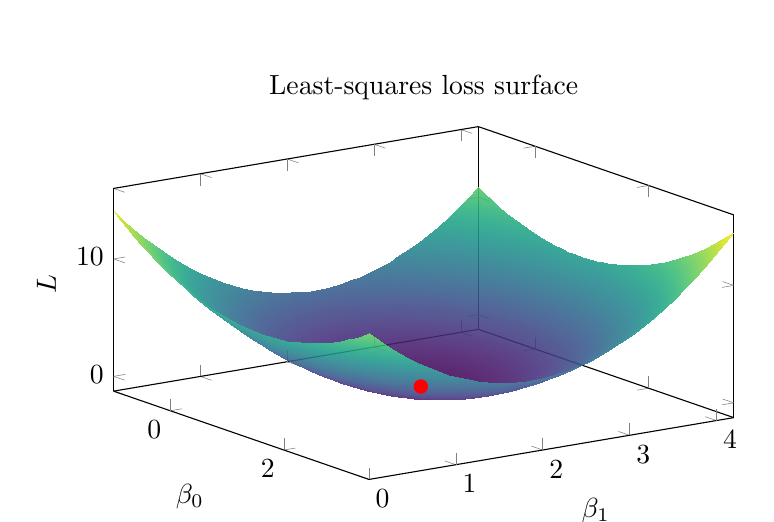
\begin{tikzpicture}
\begin{axis}[
  width=0.78\textwidth,
  height=0.50\textwidth,
  view={55}{28},
  xlabel={$\beta_0$},ylabel={$\beta_1$},zlabel={$L$},
  domain=-1:3.5,y domain=0:4.2,
  samples=38,samples y=38,
  colormap/viridis,
  z buffer=sort,
  title={Least-squares loss surface}
]
\addplot3[surf,shader=interp,opacity=0.88] {0.9*(x-1.2)^2 + 1.8*(y-2.1)^2 + 0.35*(x-1.2)*(y-2.1) + 0.18};
\addplot3[only marks,mark=*,mark size=2.4pt,red] coordinates {(1.2,2.1,0.18)};
\end{axis}
\end{tikzpicture}
\caption{A least-squares loss surface. Training searches for the lowest point in parameter space.}
\end{figure}

\begin{figure}[H]
\centering
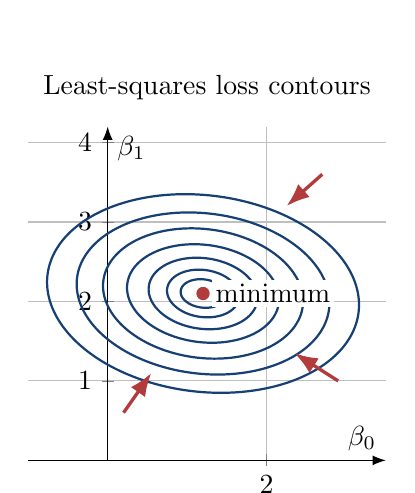
\begin{tikzpicture}
\begin{axis}[
  width=0.67\textwidth,
  height=0.48\textwidth,
  xmin=-1,xmax=3.5,ymin=0,ymax=4.2,
  axis equal image,
  axis lines=middle,
  xlabel={$\beta_0$},ylabel={$\beta_1$},
  grid=both,
  title={Least-squares loss contours},
  axis line style={-Latex}
]
\foreach \a/\b in {0.28/0.18,0.45/0.30,0.68/0.45,0.95/0.62,1.25/0.82,1.58/1.02,1.95/1.25}{
  \addplot[domain=0:360,samples=220,chapterblue!70!black,thick] ({1.2 + \a*cos(x) - .18*\b*sin(x)},{2.1 + \b*sin(x)});
}
\addplot[only marks,mark=*,mark size=2.2pt,chapterred] coordinates {(1.2,2.1)};
\node[fill=white,inner sep=1.5pt,anchor=west] at (axis cs:1.30,2.1) {minimum};
\addplot[chapterred,very thick,-Latex] coordinates {(0.2,0.6) (0.55,1.1)};
\addplot[chapterred,very thick,-Latex] coordinates {(2.7,3.6) (2.25,3.2)};
\addplot[chapterred,very thick,-Latex] coordinates {(2.9,1.0) (2.35,1.35)};
\end{axis}
\end{tikzpicture}
\caption{Contour lines of the least-squares loss. The gradient is perpendicular to the contours; the negative gradient points downhill.}
\end{figure}

\section{Matrix form and the geometry of linear models}

For multiple features, place the data in a design matrix
\[
X=\begin{bmatrix}
- & x_1\T & -\\
- & x_2\T & -\\
&\vdots&\\
- & x_n\T & -
\end{bmatrix},
\qquad
w\in\R^d,
\qquad
\widehat y=Xw.
\]
The mean squared error loss is
\[
L(w)=\frac1n\norm{Xw-y}^2.
\]
The gradient is
\[
\grad L(w)=\frac2n X\T(Xw-y).
\]
This formula is a bridge between multivariable calculus and linear algebra. The residual vector $Xw-y$ lives in data space $\R^n$, while the gradient lives in parameter space $\R^d$.

At a critical point,
\[
X\T(Xw-y)=0.
\]
Thus the residual vector is orthogonal to every column of $X$. This is the projection geometry behind least squares.

\begin{tipbox}[Geometry of least squares]
The least-squares solution chooses $Xw$ to be the orthogonal projection of $y$ onto the column space of $X$. The calculus condition $\grad L(w)=0$ is the same as the linear algebra condition that the residual is orthogonal to the model space.
\end{tipbox}

\begin{figure}[H]
\centering
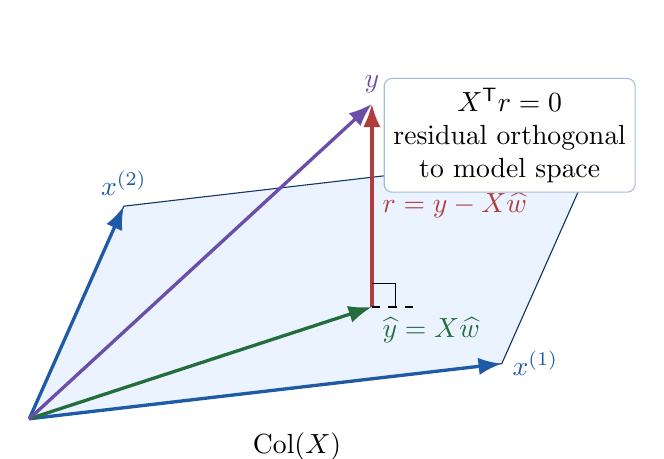
\begin{tikzpicture}[scale=1.0]
  \coordinate (O) at (0,0);
  \coordinate (A) at (6,0.7);
  \coordinate (B) at (1.2,2.7);
  \coordinate (Yhat) at (4.35,1.42);
  \coordinate (Y) at (4.35,4.0);
  \filldraw[fill=softblue,draw=chapterblue!60!black] (O) -- (A) -- ($(A)+(B)$) -- (B) -- cycle;
  \draw[vector] (O) -- (A) node[right] {$x^{(1)}$};
  \draw[vector] (O) -- (B) node[above] {$x^{(2)}$};
  \draw[very thick,chaptergreen!80!black,-Latex] (O) -- (Yhat) node[below right] {$\widehat y=X\widehat w$};
  \draw[very thick,chapterpurple,-Latex] (O) -- (Y) node[above] {$y$};
  \draw[very thick,chapterred,-Latex] (Yhat) -- (Y) node[midway,right] {$r=y-X\widehat w$};
  \draw[dashed] (Yhat) -- ++(0.55,0);
  \draw (4.35,1.72) -- (4.65,1.72) -- (4.65,1.42);
  \node at (3.4,-0.35) {$\col(X)$};
  \node[align=center,fill=white,draw=chapterblue!40,rounded corners=1mm] at (6.1,3.6) {$X\T r=0$\\residual orthogonal\\to model space};
\end{tikzpicture}
\caption{Projection geometry of least squares. The best prediction $X\widehat w$ is the projection of $y$ onto the column space of $X$.}
\end{figure}

\subsection*{Gradient descent for linear regression}

Gradient descent updates parameters by
\[
w_{k+1}=w_k-\eta\grad L(w_k),
\]
where $\eta>0$ is the learning rate. For mean squared error,
\[
w_{k+1}=w_k-\eta\frac2n X\T(Xw_k-y).
\]
If the learning rate is too small, training is slow. If it is too large, the method may oscillate or diverge.

\begin{figure}[H]
\centering
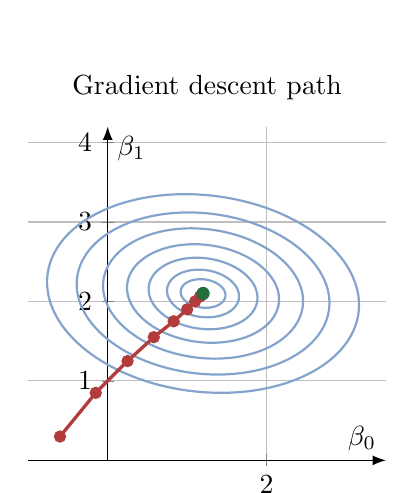
\begin{tikzpicture}
\begin{axis}[
  width=0.67\textwidth,
  height=0.48\textwidth,
  xmin=-1,xmax=3.5,ymin=0,ymax=4.2,
  axis equal image,
  axis lines=middle,
  xlabel={$\beta_0$},ylabel={$\beta_1$},
  grid=both,
  title={Gradient descent path},
  axis line style={-Latex}
]
\foreach \a/\b in {0.28/0.18,0.45/0.30,0.68/0.45,0.95/0.62,1.25/0.82,1.58/1.02,1.95/1.25}{
  \addplot[domain=0:360,samples=220,chapterblue!55,thick] ({1.2 + \a*cos(x) - .18*\b*sin(x)},{2.1 + \b*sin(x)});
}
\addplot[chapterred,very thick,mark=*,mark size=1.6pt] coordinates {(-0.6,0.3) (-0.15,0.85) (0.25,1.25) (0.58,1.55) (0.83,1.75) (1.00,1.90) (1.10,2.00) (1.16,2.06) (1.20,2.10)};
\addplot[only marks,mark=*,mark size=2.2pt,chaptergreen!80!black] coordinates {(1.2,2.1)};
\end{axis}
\end{tikzpicture}
\caption{Gradient descent follows the negative gradient direction across loss contours.}
\end{figure}

\section{Empirical risk and the structure of training problems}

Most supervised learning problems can be written as empirical risk minimization:
\[
\min_\theta L(\theta)=\min_\theta \frac1n\sum_{i=1}^n\ell(f_\theta(x_i),y_i).
\]
There are three layers:
\begin{enumerate}
  \item \textbf{Model layer:} $f_\theta(x)$ converts an input into a prediction.
  \item \textbf{Loss layer:} $\ell(f_\theta(x_i),y_i)$ measures the error on one data point.
  \item \textbf{Optimization layer:} the average loss is minimized over $\theta$.
\end{enumerate}

For a scalar-output model, the chain rule gives the gradient of one training example:
\[
\grad_\theta\ell(f_\theta(x_i),y_i)
=\frac{\partial\ell}{\partial \widehat y_i}\grad_\theta f_\theta(x_i),
\qquad \widehat y_i=f_\theta(x_i).
\]
For a vector-output model $f_\theta(x_i)\in\R^m$, the Jacobian appears:
\[
\grad_\theta\ell(f_\theta(x_i),y_i)
=J_{f_\theta}(x_i)\T\grad_{\widehat y_i}\ell(\widehat y_i,y_i).
\]
This is the central calculus identity behind backpropagation.

\begin{figure}[H]
\centering
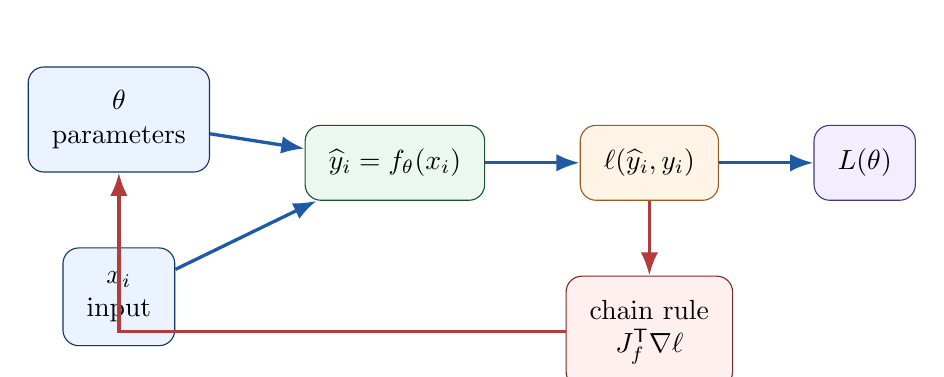
\begin{tikzpicture}[node distance=0.95cm and 1.2cm]
  \node[nodebox] (theta) {$\theta$\\parameters};
  \node[nodebox,below=of theta] (x) {$x_i$\\input};
  \node[greenbox,right=of theta,yshift=-0.55cm] (model) {$\widehat y_i=f_\theta(x_i)$};
  \node[orangebox,right=of model] (loss) {$\ell(\widehat y_i,y_i)$};
  \node[purplebox,right=of loss] (avg) {$L(\theta)$};
  \node[redbox,below=of loss] (chain) {chain rule\\$J_f\T\grad\ell$};
  \draw[vector] (theta) -- (model);
  \draw[vector] (x) -- (model);
  \draw[vector] (model) -- (loss);
  \draw[vector] (loss) -- (avg);
  \draw[descent] (loss) -- (chain);
  \draw[descent] (chain) -| (theta.south);
\end{tikzpicture}
\caption{Empirical risk has a model layer, a loss layer, and an optimization layer. The chain rule transports derivatives backward to the parameters.}
\end{figure}

\section{Logistic regression and classification}

For binary classification, labels are often $y_i\in\{0,1\}$. Logistic regression uses
\[
p_i=\sigma(w\T x_i+b),
\qquad
\sigma(z)=\frac{1}{1+e^{-z}}.
\]
The output $p_i$ is interpreted as a probability that $y_i=1$. The binary cross-entropy loss is
\[
L(w,b)=-\frac1n\sum_{i=1}^n\left[y_i\log p_i+(1-y_i)\log(1-p_i)\right].
\]
Let $z_i=w\T x_i+b$ and $p_i=\sigma(z_i)$. A useful derivative is
\[
\frac{d}{dz}\sigma(z)=\sigma(z)(1-\sigma(z)).
\]
For the cross-entropy loss, the derivative simplifies:
\[
\frac{\partial L}{\partial z_i}=\frac1n(p_i-y_i).
\]
Therefore
\[
\grad_w L(w,b)=\frac1n\sum_{i=1}^n(p_i-y_i)x_i,
\qquad
\frac{\partial L}{\partial b}=\frac1n\sum_{i=1}^n(p_i-y_i).
\]

\begin{figure}[H]
\centering
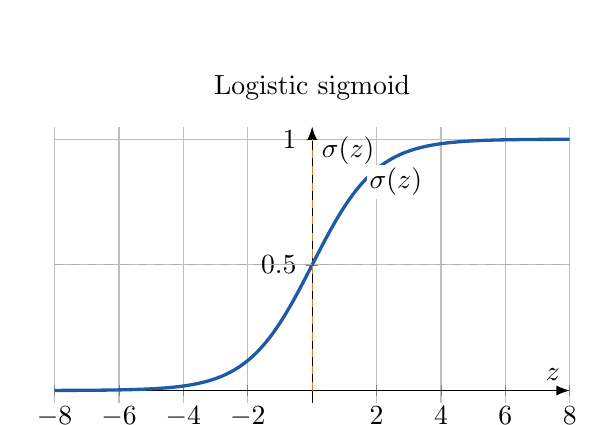
\begin{tikzpicture}
\begin{axis}[
  width=0.67\textwidth,height=0.42\textwidth,
  xmin=-8,xmax=8,ymin=-0.05,ymax=1.05,
  axis lines=middle,
  xlabel={$z$},ylabel={$\sigma(z)$},
  grid=both,
  title={Logistic sigmoid},
  axis line style={-Latex}
]
\addplot[very thick,chapterblue,domain=-8:8,samples=300] {1/(1+exp(-x))};
\addplot[dashed,gray!65] coordinates {(-8,0.5) (8,0.5)};
\addplot[dashed,chapterorange] coordinates {(0,0) (0,1)};
\node[fill=white,inner sep=1pt] at (axis cs:2.6,0.83) {$\sigma(z)$};
\end{axis}
\end{tikzpicture}
\caption{The logistic sigmoid transforms real-valued scores into probabilities between $0$ and $1$.}
\end{figure}

\begin{figure}[H]
\centering
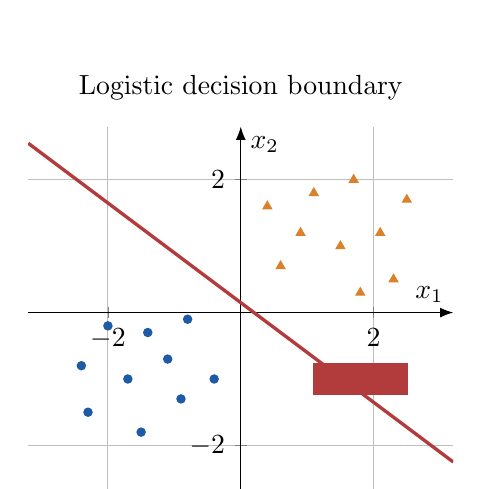
\begin{tikzpicture}
\begin{axis}[
  width=0.65\textwidth,height=0.52\textwidth,
  xmin=-3.2,xmax=3.2,ymin=-2.8,ymax=2.8,
  axis equal image,
  axis lines=middle,
  xlabel={$x_1$},ylabel={$x_2$},
  grid=both,
  title={Logistic decision boundary},
  axis line style={-Latex}
]
\addplot[only marks,mark=*,mark size=1.5pt,chapterblue] coordinates {(-2.3,-1.5)(-1.7,-1.0)(-1.4,-0.3)(-0.9,-1.3)(-1.1,-0.7)(-2.0,-0.2)(-1.5,-1.8)(-0.4,-1.0)(-2.4,-0.8)(-0.8,-0.1)};
\addplot[only marks,mark=triangle*,mark size=1.8pt,chapterorange] coordinates {(2.1,1.2)(1.5,1.0)(1.1,1.8)(0.6,0.7)(1.8,0.3)(2.5,1.7)(0.9,1.2)(1.7,2.0)(2.3,0.5)(0.4,1.6)};
\addplot[very thick,chapterred,domain=-3.2:3.2,samples=2] {-0.75*x+0.15};
\node[fill=white,inner sep=1.5pt,chapterred] at (axis cs:1.8,-1.0) {$p=0.5$};
\end{axis}
\end{tikzpicture}
\caption{A logistic regression model learns a linear decision boundary in feature space.}
\end{figure}

\section{Regularization and the bias-variance tradeoff}

A loss function measures fit to data. A regularization term measures model complexity. A common objective is
\[
J(\theta)=L(\theta)+\lambda R(\theta),
\]
where $\lambda\ge0$ controls the strength of regularization.

For ridge regression,
\[
R(w)=\norm{w}^2.
\]
The regularized objective is
\[
J(w)=\frac1n\norm{Xw-y}^2+\lambda\norm{w}^2.
\]
Its gradient is
\[
\grad J(w)=\frac2n X\T(Xw-y)+2\lambda w.
\]
The term $2\lambda w$ pulls the parameter vector toward the origin. This often improves generalization by preventing unstable parameter estimates.

\begin{mainideabox}[Calculus interpretation of regularization]
Regularization changes the geometry of the loss surface. It adds curvature that penalizes large parameter values, often making the optimization problem better conditioned.
\end{mainideabox}

\begin{figure}[H]
\centering
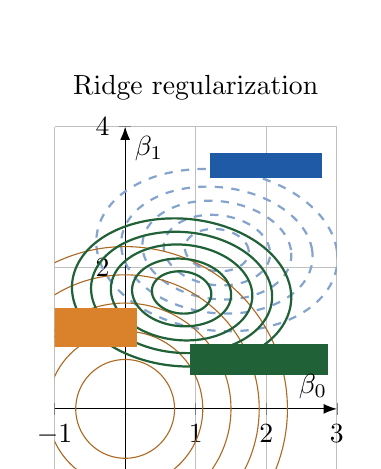
\begin{tikzpicture}
\begin{axis}[
  width=0.67\textwidth,height=0.50\textwidth,
  xmin=-1,xmax=3,ymin=-1,ymax=4,
  axis equal image,
  axis lines=middle,
  xlabel={$\beta_0$},ylabel={$\beta_1$},
  grid=both,
  title={Ridge regularization},
  axis line style={-Latex}
]
\foreach \a/\b in {0.45/0.30,0.75/0.50,1.05/0.70,1.35/0.90,1.7/1.15}{
  \addplot[domain=0:360,samples=180,chapterblue!55,dashed,thick] ({1.3 + \a*cos(x)-0.15*\b*sin(x)},{2.25 + \b*sin(x)});
}
\foreach \r in {0.7,1.1,1.5,1.9,2.3}{
  \addplot[domain=0:360,samples=180,chapterorange!80!black,thin] ({\r*cos(x)},{\r*sin(x)});
}
\foreach \a/\b in {0.42/0.30,0.70/0.48,1.0/0.68,1.28/0.86,1.55/1.05}{
  \addplot[domain=0:360,samples=180,chaptergreen!70!black,thick] ({0.8 + \a*cos(x)-0.10*\b*sin(x)},{1.65 + \b*sin(x)});
}
\node[fill=white,inner sep=1pt,chapterblue] at (axis cs:2.0,3.45) {data loss};
\node[fill=white,inner sep=1pt,chapterorange] at (axis cs:-0.45,1.15) {$\lambda\norm{w}^2$};
\node[fill=white,inner sep=1pt,chaptergreen!70!black] at (axis cs:1.9,0.7) {regularized};
\end{axis}
\end{tikzpicture}
\caption{Ridge regularization adds circular penalty contours to the data-fitting loss, shifting the optimum toward smaller coefficients.}
\end{figure}

\section{Stochastic gradient descent}

For large data sets, computing the full gradient
\[
\grad L(\theta)=\frac1n\sum_{i=1}^n\grad_\theta\ell_i(\theta)
\]
may be expensive. Stochastic gradient descent replaces the full average by a random estimate:
\[
\theta_{k+1}=\theta_k-\eta_k g_k,
\]
where $g_k$ is computed from one data point or a mini-batch. A mini-batch gradient has the form
\[
g_k=\frac{1}{\abs{B_k}}\sum_{i\in B_k}\grad_\theta\ell_i(\theta_k).
\]
This introduces noise into the path. The noise can slow convergence near a minimum, but it can also help training move through complicated landscapes.

\begin{figure}[H]
\centering
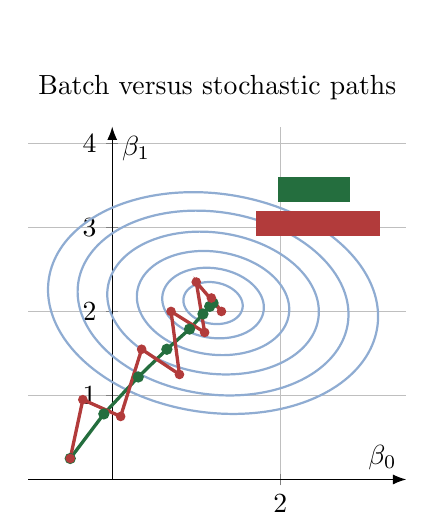
\begin{tikzpicture}
\begin{axis}[
  width=0.67\textwidth,height=0.50\textwidth,
  xmin=-1,xmax=3.5,ymin=0,ymax=4.2,
  axis equal image,
  axis lines=middle,
  xlabel={$\beta_0$},ylabel={$\beta_1$},
  grid=both,
  title={Batch versus stochastic paths},
  axis line style={-Latex}
]
\foreach \a/\b in {0.35/0.25,0.60/0.42,0.90/0.62,1.25/0.85,1.60/1.10,1.95/1.32}{
  \addplot[domain=0:360,samples=180,chapterblue!50,thick] ({1.2 + \a*cos(x)-0.18*\b*sin(x)},{2.1 + \b*sin(x)});
}
\addplot[chaptergreen!80!black,very thick,mark=*,mark size=1.4pt] coordinates {(-0.5,0.25)(-0.1,0.78)(0.31,1.22)(0.65,1.55)(0.92,1.79)(1.08,1.97)(1.16,2.06)(1.2,2.1)};
\addplot[chapterred,very thick,mark=*,mark size=1.1pt] coordinates {(-0.5,0.25)(-0.35,0.95)(0.1,0.75)(0.35,1.55)(0.8,1.25)(0.7,2.0)(1.1,1.75)(1.0,2.35)(1.3,2.0)(1.18,2.16)};
\node[fill=white,inner sep=1pt,chaptergreen!80!black] at (axis cs:2.4,3.45) {batch};
\node[fill=white,inner sep=1pt,chapterred] at (axis cs:2.45,3.05) {stochastic};
\end{axis}
\end{tikzpicture}
\caption{Batch gradient descent follows a smooth path; stochastic gradient descent follows a noisier path.}
\end{figure}

\section{Neural networks and the chain rule}

A neural network is a composition of functions. A simple one-hidden-layer network has the form
\[
f_\theta(x)=W_2\,\phi(W_1x+b_1)+b_2,
\]
where $\phi$ is an activation function applied componentwise. The parameters are
\[
\theta=(W_1,b_1,W_2,b_2).
\]
The main calculus idea is not new: the derivative of a composition is computed by the chain rule. What changes is scale. A network may have many layers:
\[
x\mapsto h_1\mapsto h_2\mapsto\cdots\mapsto h_K\mapsto \widehat y\mapsto L.
\]
Backpropagation computes derivatives from the output backward through the computational graph.

\begin{figure}[H]
\centering
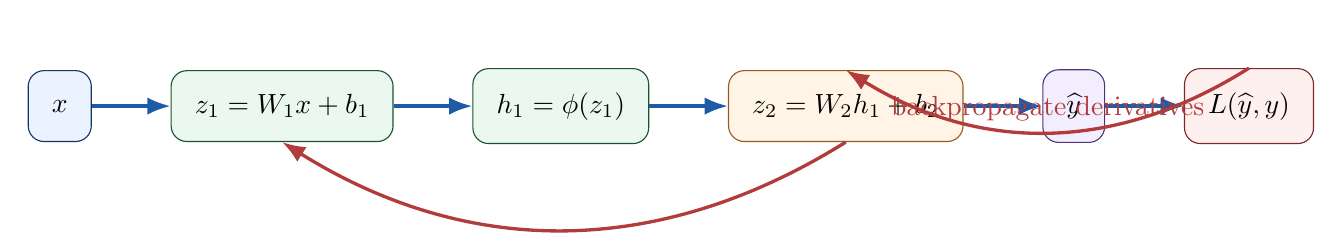
\begin{tikzpicture}[node distance=1.0cm and 1.0cm]
  \node[nodebox] (x) {$x$};
  \node[greenbox,right=of x] (z1) {$z_1=W_1x+b_1$};
  \node[greenbox,right=of z1] (h1) {$h_1=\phi(z_1)$};
  \node[orangebox,right=of h1] (z2) {$z_2=W_2h_1+b_2$};
  \node[purplebox,right=of z2] (yhat) {$\widehat y$};
  \node[redbox,right=of yhat] (loss) {$L(\widehat y,y)$};
  \draw[vector] (x) -- (z1);
  \draw[vector] (z1) -- (h1);
  \draw[vector] (h1) -- (z2);
  \draw[vector] (z2) -- (yhat);
  \draw[vector] (yhat) -- (loss);
  \draw[descent,bend left=32] (loss.north) to node[above] {backpropagate derivatives} (z2.north);
  \draw[descent,bend left=32] (z2.south) to (z1.south);
\end{tikzpicture}
\caption{A neural network is a composition. Backpropagation is the chain rule applied backward through the computational graph.}
\end{figure}

\subsection*{A scalar example}

Let
\[
\widehat y=a\,\phi(wx+b),
\qquad
L=\frac12(\widehat y-y)^2.
\]
Let $z=wx+b$ and $h=\phi(z)$. Then $\widehat y=ah$. By the chain rule,
\[
\frac{\partial L}{\partial a}=(\widehat y-y)h,
\]
\[
\frac{\partial L}{\partial w}=(\widehat y-y)a\phi'(z)x,
\]
and
\[
\frac{\partial L}{\partial b}=(\widehat y-y)a\phi'(z).
\]
Every large backpropagation computation is built from this same pattern.

\begin{figure}[H]
\centering
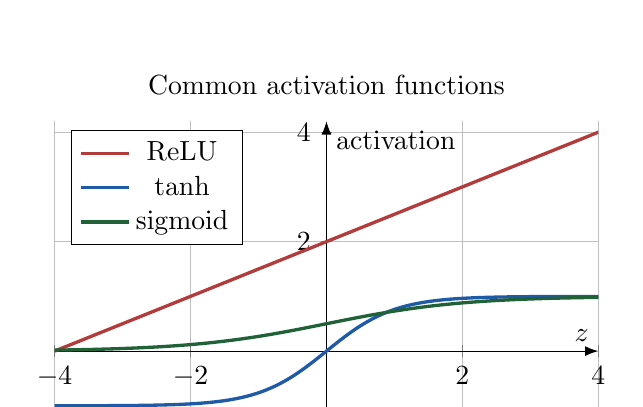
\begin{tikzpicture}
\begin{axis}[
  width=0.70\textwidth,height=0.44\textwidth,
  xmin=-4,xmax=4,ymin=-1.2,ymax=4.2,
  axis lines=middle,
  xlabel={$z$},ylabel={activation},
  grid=both,
  title={Common activation functions},
  legend style={at={(0.03,0.97)},anchor=north west,fill=white},
  axis line style={-Latex}
]
\addplot[very thick,chapterred,domain=-4:4,samples=2] {max(0,x)};
\addlegendentry{ReLU}
\addplot[very thick,chapterblue,domain=-4:4,samples=300] {tanh(x)};
\addlegendentry{$\tanh$}
\addplot[very thick,chaptergreen!70!black,domain=-4:4,samples=300] {1/(1+exp(-x))};
\addlegendentry{sigmoid}
\end{axis}
\end{tikzpicture}
\caption{Common activation functions shape how neural networks bend space.}
\end{figure}

\section{Numerical gradient checking}

Even when gradients are computed automatically, it is useful to understand numerical checks. For a differentiable function $L:\R^p\to\R$, the central difference approximation to the $j$th partial derivative is
\[
\frac{\partial L}{\partial \theta_j}(\theta)
\approx
\frac{L(\theta+h e_j)-L(\theta-h e_j)}{2h}.
\]
This checks whether an analytic or automatic gradient is plausible.

\begin{figure}[H]
\centering
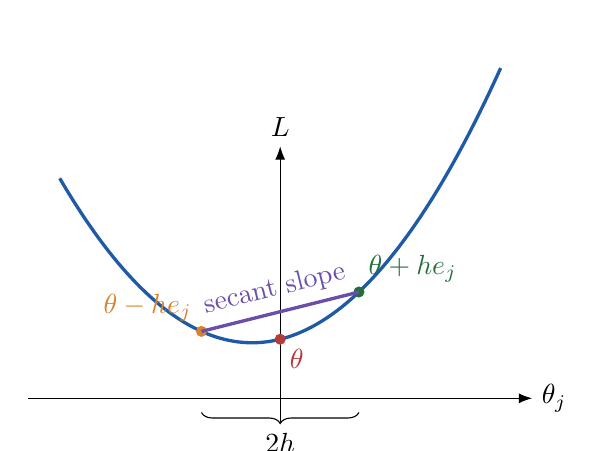
\begin{tikzpicture}[scale=1.0]
  \draw[-Latex] (-3.2,0) -- (3.2,0) node[right] {$\theta_j$};
  \draw[-Latex] (0,-0.3) -- (0,3.2) node[above] {$L$};
  \draw[very thick,chapterblue,domain=-2.8:2.8,samples=100] plot (\x,{0.35*(\x)^2+0.25*\x+0.75});
  \coordinate (M) at (0,0.75);
  \coordinate (P) at (1,1.35);
  \coordinate (N) at (-1,0.85);
  \fill[chapterred] (M) circle (2pt) node[below right] {$\theta$};
  \fill[chaptergreen!80!black] (P) circle (2pt) node[above right] {$\theta+h e_j$};
  \fill[chapterorange] (N) circle (2pt) node[above left] {$\theta-h e_j$};
  \draw[chapterpurple,very thick] (N) -- (P) node[midway,above,sloped] {secant slope};
  \draw[decorate,decoration={brace,mirror,amplitude=4pt}] (-1,-0.18) -- (1,-0.18) node[midway,below=4pt] {$2h$};
\end{tikzpicture}
\caption{A central difference uses two nearby function values to approximate one component of the gradient.}
\end{figure}

A small difference between the analytic and numerical gradients gives confidence that the derivative was implemented correctly. A large difference suggests an algebra error, a coding error, or a nondifferentiability issue.

\section{Hessians, curvature, and learning rates}

Near a point $\theta_0$, a twice differentiable loss has the second-order approximation
\[
L(\theta_0+u)\approx L(\theta_0)+\grad L(\theta_0)\T u+\frac12 u\T H_L(\theta_0)u.
\]
The Hessian tells us how curved the loss is in different directions. If the Hessian has eigenvalues with very different sizes, the level sets are long and narrow. Gradient descent may zigzag.

For least squares,
\[
L(w)=\frac1n\norm{Xw-y}^2,
\]
the Hessian is constant:
\[
H_L(w)=\frac2n X\T X.
\]
The eigenvalues of $X\T X$ control the conditioning of the optimization problem.

\begin{figure}[H]
\centering
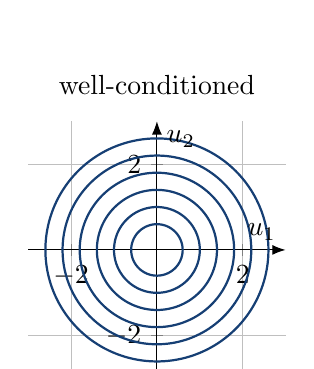
\begin{tikzpicture}
\begin{axis}[
  width=0.44\textwidth,height=0.40\textwidth,
  xmin=-3,xmax=3,ymin=-3,ymax=3,
  axis equal image,
  axis lines=middle,
  xlabel={$u_1$},ylabel={$u_2$},
  title={well-conditioned},
  grid=both,
  axis line style={-Latex}
]
\foreach \r in {.6,1.0,1.4,1.8,2.2,2.6}{
  \addplot[domain=0:360,samples=160,chapterblue!70!black,thick] ({\r*cos(x)},{\r*sin(x)});
}
\end{axis}
\end{tikzpicture}
\hfill
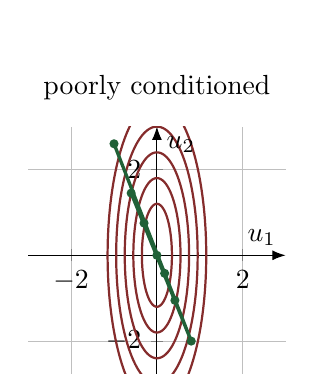
\begin{tikzpicture}
\begin{axis}[
  width=0.44\textwidth,height=0.40\textwidth,
  xmin=-3,xmax=3,ymin=-3,ymax=3,
  axis equal image,
  axis lines=middle,
  xlabel={$u_1$},ylabel={$u_2$},
  title={poorly conditioned},
  grid=both,
  axis line style={-Latex}
]
\foreach \a/\b in {.35/1.2,.55/1.8,.75/2.4,.95/3.0,1.15/3.6}{
  \addplot[domain=0:360,samples=160,chapterred!75!black,thick] ({\a*cos(x)},{\b*sin(x)});
}
\addplot[chaptergreen!70!black,very thick,mark=*,mark size=1pt] coordinates {(-1.0,2.6)(0.8,-2.0)(-0.6,1.45)(0.42,-1.05)(-0.3,0.75)(0.18,-0.42)(0.0,0.0)};
\end{axis}
\end{tikzpicture}
\caption{Poor conditioning creates narrow valleys, making gradient descent sensitive to learning rate and prone to zigzagging.}
\end{figure}

\section{Feature maps and nonlinear models}

A model can be nonlinear in the input but linear in parameters. For example,
\[
f_w(x)=w_0+w_1x+w_2x^2.
\]
This is linear regression after replacing $x$ by the feature vector
\[
\phi(x)=(1,x,x^2).
\]
More generally, a feature map
\[
\phi:\R^d\to\R^m
\]
transforms the original input into a space where a simpler model may work better.

\begin{figure}[H]
\centering
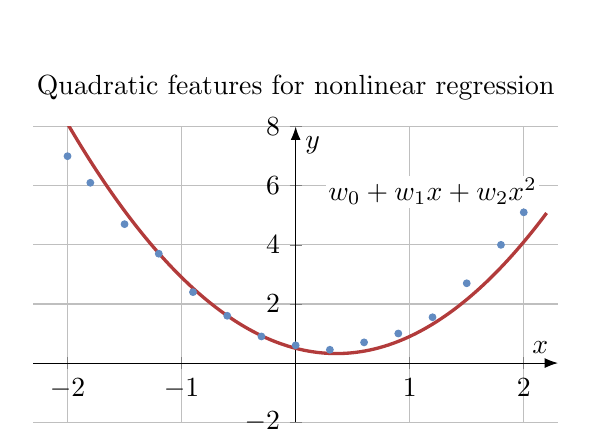
\begin{tikzpicture}
\begin{axis}[
  width=0.68\textwidth,height=0.44\textwidth,
  xmin=-2.3,xmax=2.3,ymin=-2,ymax=8,
  axis lines=middle,
  xlabel={$x$},ylabel={$y$},
  grid=both,
  title={Quadratic features for nonlinear regression},
  axis line style={-Latex}
]
\addplot[only marks,mark=*,mark size=1.2pt,chapterblue!70] coordinates {(-2.0,7.0)(-1.8,6.1)(-1.5,4.7)(-1.2,3.7)(-0.9,2.4)(-0.6,1.6)(-0.3,0.9)(0.0,0.6)(0.3,0.45)(0.6,0.7)(0.9,1.0)(1.2,1.55)(1.5,2.7)(1.8,4.0)(2.0,5.1)};
\addplot[very thick,chapterred,domain=-2.2:2.2,samples=200] {0.5 - 1.0*x + 1.4*x^2};
\node[fill=white,inner sep=1pt] at (axis cs:1.2,5.8) {$w_0+w_1x+w_2x^2$};
\end{axis}
\end{tikzpicture}
\caption{A nonlinear feature map can turn a curved pattern into a linear problem in transformed coordinates.}
\end{figure}

This example separates two ideas:
\begin{itemize}
  \item \emph{nonlinear in the input} means the graph may bend;
  \item \emph{linear in the parameters} means the loss may still be a convex quadratic.
\end{itemize}
Neural networks are more complicated because they are usually nonlinear in both inputs and parameters.

\section{What calculus tells us about machine learning}

Multivariable calculus gives a precise language for several major questions in machine learning.

\subsection*{Sensitivity}
How much does the output change when the input or parameters change? This is measured by derivatives and Jacobians.

\subsection*{Training}
How should parameters be changed to reduce the loss? This is guided by gradients and optimization algorithms.

\subsection*{Curvature}
Why is one learning problem easy and another hard? Hessians, eigenvalues, and conditioning provide part of the answer.

\subsection*{Generalization}
Why might a model fit training data but fail on new data? Regularization, model complexity, and stability are connected to the geometry of the parameter space.

\subsection*{Computation}
How can derivatives be computed for huge composed functions? The answer is the chain rule organized as automatic differentiation.

\begin{summarybox}[The big picture]
Machine learning does not replace calculus. It scales calculus. The same gradient, Jacobian, Hessian, and chain-rule ideas from this book become computational tools for learning from data.
\end{summarybox}

\section{Common mistakes}

\begin{warningbox}[Common mistakes]
\begin{enumerate}
  \item \textbf{Confusing feature space and parameter space.} Inputs $x$ live in feature space; parameters $\theta$ live in parameter space. Gradients of the loss are usually taken with respect to parameters.
  \item \textbf{Using the gradient direction instead of the negative gradient direction.} The gradient points toward steepest increase. Gradient descent moves in the negative gradient direction.
  \item \textbf{Choosing a learning rate without checking behavior.} A learning rate can be too small, useful, unstable, or divergent.
  \item \textbf{Assuming every loss is convex.} Least squares is convex in linear parameters, but neural-network losses are usually nonconvex.
  \item \textbf{Ignoring scaling.} Feature scaling changes the geometry of the loss surface and can strongly affect optimization.
  \item \textbf{Trusting code without gradient checks.} Numerical derivatives are useful for debugging small models.
\end{enumerate}
\end{warningbox}

\section{Practice problems}

\subsection*{Conceptual problems}
\begin{enumerate}
  \item Explain the difference between feature space and parameter space for a linear model $f_w(x)=w\T x$.
  \item What does the loss surface represent in linear regression?
  \item Why is the negative gradient direction used in gradient descent?
  \item Explain why the chain rule is the mathematical foundation of backpropagation.
  \item In logistic regression, why is the output interpreted as a probability?
  \item What is the purpose of regularization?
  \item Why can poor conditioning slow down gradient descent?
  \item What is the difference between batch gradient descent and stochastic gradient descent?
\end{enumerate}

\subsection*{Computational problems}
\begin{enumerate}[start=9]
  \item For $L(w_1,w_2)=3w_1^2+2w_1w_2+w_2^2$, compute $\grad L$ and perform three steps of gradient descent starting at $(1,2)$ with learning rate $\eta=0.1$.
  \item Let
  \[
  L(\beta_0,\beta_1)=\frac13\left[(1-\beta_0)^2+(2-\beta_0-\beta_1)^2+(4-\beta_0-2\beta_1)^2\right].
  \]
  Compute $\grad L$ and solve $\grad L=0$.
  \item For logistic regression with one feature, $p_i=\sigma(wx_i+b)$, show that
  \[
  \frac{\partial L}{\partial w}=\frac1n\sum_{i=1}^n(p_i-y_i)x_i.
  \]
  \item For ridge regression,
  \[
  J(w)=\frac1n\norm{Xw-y}^2+\lambda\norm{w}^2,
  \]
  compute the Hessian.
  \item Let $f_w(x)=w_0+w_1x+w_2x^2$. Write the design matrix for data points $x_1,\ldots,x_n$.
  \item Suppose $L(\theta)=\frac12(f(\theta)-y)^2$. Show that
  \[
  \grad L(\theta)=(f(\theta)-y)\grad f(\theta).
  \]
\end{enumerate}

\subsection*{Python problems}
\begin{enumerate}[start=15]
  \item Modify the gradient descent code in this chapter to use a smaller learning rate and compare the path.
  \item Modify the logistic regression simulation so that the two classes overlap more. What happens to the decision boundary?
  \item Implement ridge regression by gradient descent and compare the result for $\lambda=0$, $\lambda=0.1$, and $\lambda=1$.
  \item Write a numerical gradient checker for the logistic regression loss.
  \item Simulate stochastic gradient descent with different mini-batch sizes.
  \item Create a polynomial regression example with features $1,x,x^2,x^3$ and compare the fit to a linear model.
\end{enumerate}

\subsection*{Project problems}
\begin{enumerate}[start=21]
  \item \textbf{Loss landscape project.} Choose a two-parameter model and create a contour plot of its loss surface. Overlay several gradient descent paths with different learning rates.
  \item \textbf{Classification project.} Generate a two-class data set, train logistic regression from scratch, and visualize the learned decision boundary.
  \item \textbf{Regularization project.} Fit polynomial models of several degrees and compare training error, testing error, and coefficient size.
  \item \textbf{Backpropagation project.} Implement the scalar neural-network example from Section 25.8 and compare analytic gradients with numerical gradients.
\end{enumerate}

\section{Python lab and interactive page}

\begin{itemize}
  \item Notebook lab: \texttt{Chapter25\_Multivariable\_Calculus\_for\_Data\_Science\_and\_Machine\_Learning.ipynb}
  \item Interactive page: \texttt{chapter-25.html}
\end{itemize}

\section{Chapter summary}

This chapter connected multivariable calculus to data science and machine learning. A model is a function with parameters, and training is the problem of minimizing a loss function on parameter space. Gradients guide local improvement, Hessians describe curvature, Jacobians measure sensitivity, and the chain rule powers backpropagation. Linear regression, logistic regression, regularization, stochastic gradient descent, and neural networks all use the same core calculus ideas developed throughout this book.

\end{document}
